\documentclass[a4paper,twoside]{article}
\usepackage[inner=16mm,outer=16mm,top=18mm,bottom=17mm,headheight=12pt,headsep=5mm,footskip=8mm]{geometry}
\usepackage{fontspec}
\setmainfont{Liberation Serif}
\setsansfont{Liberation Sans}
\setmonofont[Scale=.88]{Liberation Mono}
\usepackage[table]{xcolor}
\definecolor{ruleblue}{HTML}{00649A}
\definecolor{coverpaper}{HTML}{C6C0AE}
\definecolor{coverink}{HTML}{792D2A}
\definecolor{notepaper}{HTML}{E8EEF4}
\usepackage{graphicx,multicol,booktabs,array,amsmath,amssymb,enumitem,needspace,titlesec,fancyhdr,microtype}
\usepackage[breakable,skins]{tcolorbox}
\usepackage{xurl}
\usepackage{hyperref}
\hypersetup{unicode=true,hidelinks,pdftitle={$title$ — Rules of Play},pdfauthor={Research prototype},pdfsubject={Scenario A; ruleset R3; A4 portrait}}
\setlength{\columnsep}{6mm}
\setlength{\parindent}{0pt}
\setlength{\parskip}{3pt plus .3pt minus .3pt}
\setlength{\emergencystretch}{1em}
\setlist{nosep,leftmargin=12pt,topsep=3pt,parsep=1pt}
\setcounter{secnumdepth}{0}
\setcounter{tocdepth}{1}
\titleformat{\section}{\sffamily\bfseries\color{ruleblue}\fontsize{13}{14}\selectfont}{}{0pt}{}
\titleformat{\subsection}{\sffamily\bfseries\fontsize{10.5}{11.5}\selectfont}{}{0pt}{}
\titleformat{\subsubsection}{\bfseries\fontsize{9.5}{10.7}\selectfont}{}{0pt}{}
\titlespacing*{\section}{0pt}{8pt}{4pt}
\titlespacing*{\subsection}{0pt}{7pt}{3pt}
\titlespacing*{\subsubsection}{0pt}{5pt}{2pt}
\newtcolorbox{rulenote}{enhanced,breakable,colback=notepaper,colframe=notepaper,boxrule=0pt,arc=0pt,left=4pt,right=4pt,top=3pt,bottom=3pt,before skip=4pt,after skip=4pt}
\renewenvironment{quote}{\begin{rulenote}\itshape}{\end{rulenote}}
\providecommand{\tightlist}{\setlength{\itemsep}{0pt}\setlength{\parskip}{0pt}}
\pagestyle{fancy}
\fancyhf{}
\fancyhead[LE,RO]{\sffamily\fontsize{8}{9}\selectfont\thepage}
\fancyhead[CE,CO]{\sffamily\itshape\fontsize{8}{9}\selectfont A Handful of Bandits\quad\textcolor{ruleblue}{Scenario A · R3}}
\fancyfoot[C]{\sffamily\fontsize{7}{8}\selectfont Research prototype · 31 October 2026 · Rules of Play}
\renewcommand{\headrulewidth}{.4pt}
\renewcommand{\footrulewidth}{0pt}
\begin{document}
\fontsize{9.5}{10.7}\selectfont
\begin{titlepage}
\pagecolor{coverpaper}\thispagestyle{empty}
\centering
\vspace*{2mm}
{\fontsize{35}{38}\selectfont\bfseries\color{coverink} A Handful of Bandits\par}
\vspace{4mm}
{\sffamily\bfseries\fontsize{15}{18}\selectfont Turkey and the PKK, 1984–1989\par}
\vspace{6mm}
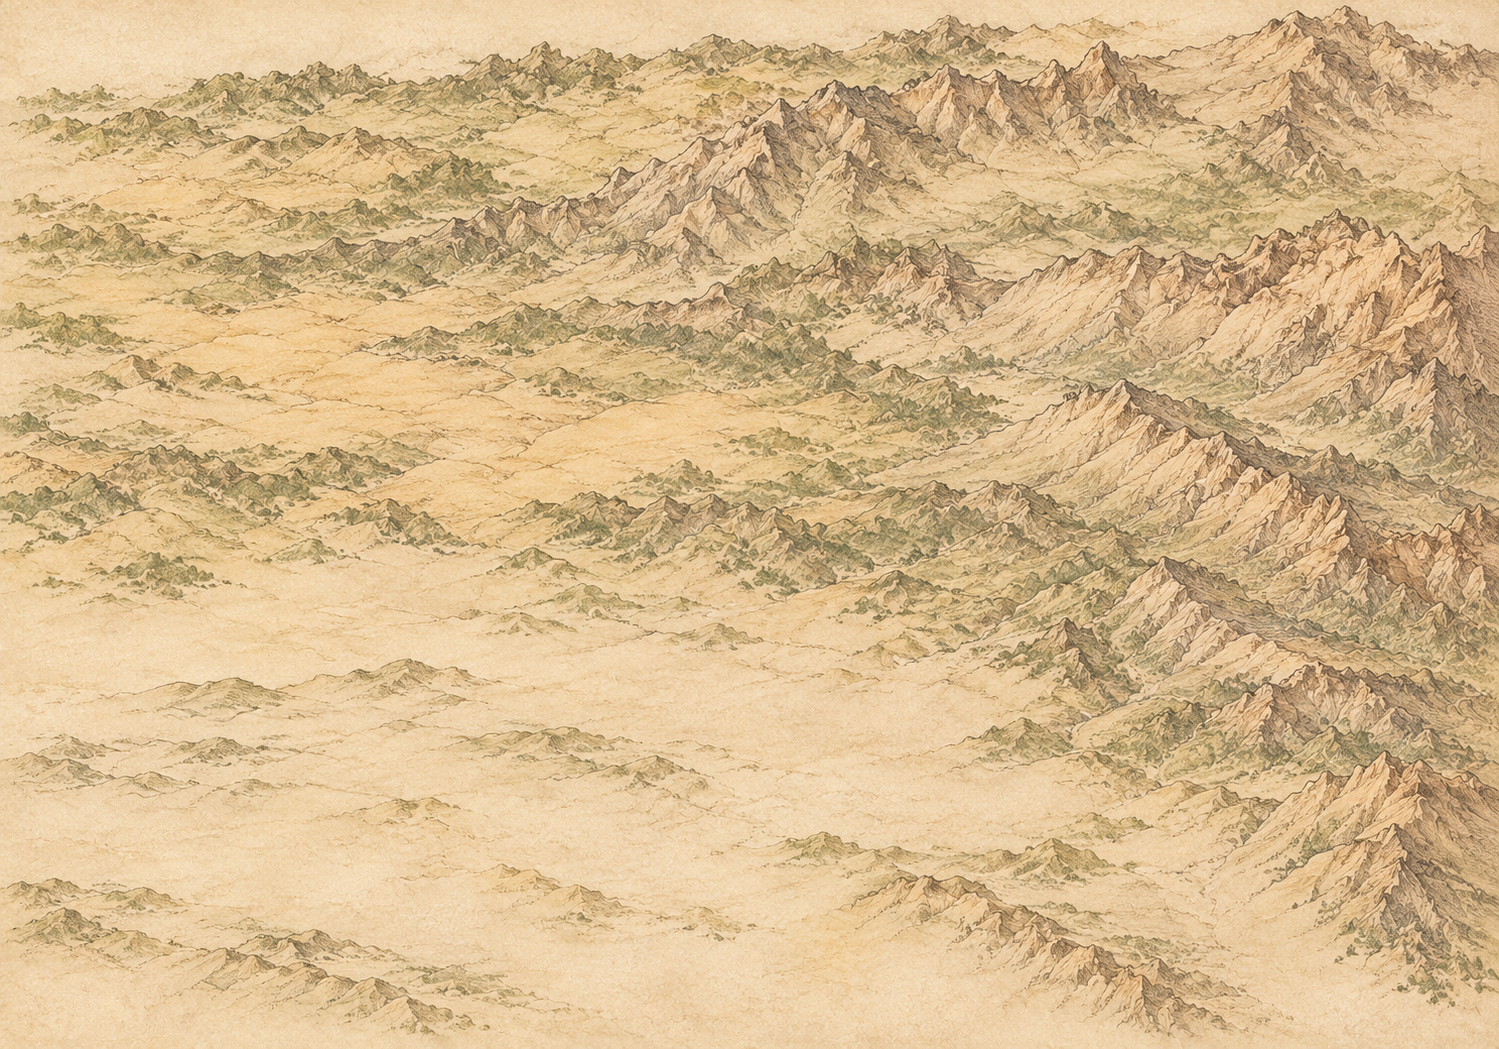
\includegraphics[width=\textwidth,height=80mm]{../../game-packages/kurdish-coin/0.1.0/map/atlas-terrain.png}
\vspace{5mm}
{\sffamily\bfseries\fontsize{11}{13}\selectfont SCENARIO A · C1/C2 · RULESET R3\par}
\vspace{4mm}
{\fontsize{29}{32}\selectfont R U L E S\; O F\; P L A Y\par}
\vspace{3mm}
{\sffamily\fontsize{10}{12}\selectfont Playable research prototype · 31 October 2026\par}
\vspace{4mm}
\begin{tcolorbox}[colback=white!48!coverpaper,colframe=white,arc=0pt,boxrule=.7pt,left=8mm,right=8mm,top=4mm,bottom=4mm]
{\centering\sffamily\bfseries\fontsize{10}{12}\selectfont T A B L E\; O F\; C O N T E N T S\par}
\vspace{2mm}
\makeatletter
{\fontsize{9}{11}\selectfont\begin{multicols}{2}\@starttoc{toc}\end{multicols}}
\makeatother
\end{tcolorbox}
\vfill
{\sffamily\fontsize{8}{10}\selectfont A4 portrait · Print at 100\% / Actual size\par}
{\sffamily\fontsize{8}{10}\selectfont Prototype rules, not an official COIN-series publication\par}
\end{titlepage}
\nopagecolor
\setcounter{page}{2}
\begin{multicols}{2}
\raggedcolumns
$body$
\end{multicols}
\end{document}
